\section{Stirling approximation}
\begin{equation}
n!=\Gamma(n+1) \approx S(n) = n^n e^{-n} \sqrt{\pi \left(2n+\frac{1}{3}\right)}
\end{equation}
Note the $+\frac{1}{3}$ is usually omitted, but including the term makes a better asymptotic approximation, and it matches 0!=1 much better than without this term.

\begin{figure}
  \caption{Stirling (modified) $S(n)$ (red) vs Stirling (unmodified blue) vs. $\Gamma(n+1)$ (green)}
  \centering
    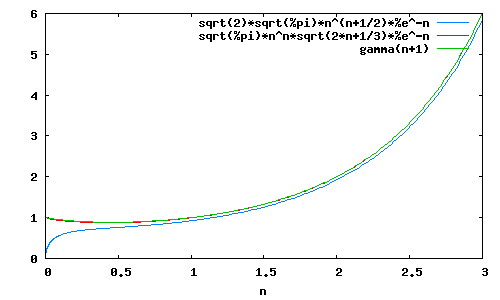
\includegraphics[width=1.0\textwidth]{stirling}
\end{figure}
